\chapter{Near-Optimal Glimpse Sequences for Improved Hard Attention Neural Network Training }

\section{Introduction}
\label{sec:nogs-introduction}
In humans, the density of photoreceptors varies across the retina; it is much
greater in the centre~\cite{bear2007neuroscience} and covers an approximately
210 degree field of view~\cite{traquair1949introduction}. The visual system is
therefore a limited resource with respect to observing the environment and it
must be allocated, or controlled, by some attention mechanism. We refer to this
kind of controlled allocation of limited sensor resources as ``hard'' attention.
This is in contrast with ``soft'' attention, the controlled application of
limited computational resources to full sensory input. Hard attention can solve
certain tasks using orders of magnitude less sensor bandwidth and computation
than the alternatives~\cite{katharopoulos2019processing, rensink2000dynamic}.
It therefore may enable the use of modern approaches to computer vision in
low-power mobile devices and integrated circuits.

\begin{figure*}[t]
  \centering
  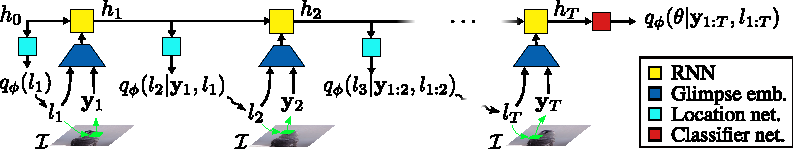
\includegraphics[scale=1]{figs/nogs/hard-attention-architecture}
  \caption{The hard attention network architecture we consider, consisting of an
    RNN core (yellow), a location network (light blue), a glimpse embedder (dark
    blue), and a classifier (red). We use $h_t$ to denote the RNN hidden state
    after $t$ steps. At each step, the location network outputs a distribution
    over attention locations, from which $l_t$ is sampled. After $T$ steps, the
    classifier network outputs a distribution over the class label $\theta$ and
    the process terminates. }
  \label{fig:hard-attention-architecture}
\end{figure*}

This paper focuses on the application of hard attention to image classification.
Our model of attention (shown in \lref{fig:hard-attention-architecture}) is as
follows: a recurrent neural network (RNN) is given $T$ steps to classify some
unchanging input image. Before each step, the RNN outputs the coordinates of a
pixel in the image. A patch of the image centered around this pixel is then fed
into the RNN. We call this image patch a glimpse, and the coordinates a glimpse
location. As such, the RNN controls its input by selecting each glimpse
location, and this decision can be based on previous glimpses. After $T$ steps,
the RNN's hidden state is mapped to a classification output. As with most
artificial hard attention mechanisms~\cite{mnih2014recurrent,ba2014multiple},
this output is not differentiable with respect to the sequence of glimpse
locations selected. This makes training with standard gradient backpropagation
impossible, and so high variance gradient estimators such as
REINFORCE~\cite{williams1992simple} are commonly used
instead~\cite{mnih2014recurrent,ba2014multiple}. The resulting noisy gradient
estimates make training difficult, especially for large $T$.

We circumvent this problem by introducing supervision in the form of targets for
where the network should attend at each time step. By creating such supervision
sequences, and using them in training with the loss we introduce in
\cref{sec:nogs-partially-supervised-training}, a hard attention network can be
trained without noisy REINFORCE-style gradient estimates. We suggest two methods
for generating supervision sequences. One is to train a hard attention network
for a given task using REINFORCE and then record the sequences of locations
attended to by this network on the training data. These can be used to
supervise, and therefore speed up, the training of later networks. We call the
method of training with these supervision sequences \PSRAM{} (partial
supervision by a recurrent attention model).

Although \PSRAM{} greatly speeds up training, these supervision sequences can be
unintuitive and lead to sub-optimal training outcomes. We therefore propose an
alternative inspired by suggestions in the neuroscience literature that visual
attention is directed so as to maximally reduce entropy in an agent's world
model~\cite{bruce2009saliency, itti2009bayesian, schwartenbeck2013exploration,
  feldman2010attention}. There is a corresponding mathematical formulation of
such an objective, namely Bayesian optimal experimental design (BOED)
\cite{chaloner1995bayesian}. BOED tackles the problem of designing an
experiment to maximally reduce uncertainty in some unknown variable. When
classifying an image with hard visual attention, the `experiment' is the process
of taking a glimpse; the `design' is the glimpse location; and the unknown
variable is the class label. In general, BOED is applicable only when a
probabilistic model of the experiment exists. We leverage generative adversarial
networks (GANs)~\cite{goodfellow2014generative} to provide the required model
of the image distribution. We use methodology from BOED to create `near-optimal'
supervision sequences, and denote the method of training with these \PSNOGS{}
(partial supervision by near-optimal glimpse sequences).

We empirically investigate the performance of \PSRAM{} and \PSNOGS{}. Both lead
to faster training than our baselines. \PSNOGS{} gives particular improvements
in training speed, and leads to networks exhibiting qualitatively different
behaviour than the baselines, with competitive accuracy. We use \PSNOGS{} in a
search over hard attention architectures, and find that hard attention can
outperform conventional methods when the available computational resources are
limited.

\section{Hard Attention} \label{sec:nogs-hard-attention}
Given an image, $\x$, we consider the task of inferring its label, $\theta$. We
use an architecture based on that of \cite{mnih2014recurrent}, shown in
\lref{fig:hard-attention-architecture}. It runs for a fixed number of steps,
$T$. At each step $t$,
%
the RNN samples a glimpse location, $l_t$, from a distribution conditioned on
previous glimpses via the RNN's hidden state. A glimpse, in the form of a
contiguous square of pixels, is extracted from the image at this location. We
denote this $\y_t = \fovea(\x, l_t)$. An embedding of $\y_t$ and $l_t$ is then
input to the RNN.
%
After $T$ glimpses, the network outputs a classification distribution
$q_\phi(\theta|\y_{1:T},l_{1:T})$, where $\phi$ are the learnable network
parameters. \cite{mnih2014recurrent} use glimpses consisting of three image
patches at different resolutions, but the architectures are otherwise identical.
As it directly processes only a fraction of an image, this architecture is
suited to low-power scenarios such as use on mobile devices.

During optimisation, gradients cannot be computed by simple backpropagation
since $\fovea$ is non-differentiable with respect to the choice of location. An
alternative, taken by \cite{mnih2014recurrent} and others in the
literature~\cite{ba2014multiple,sermanet2014attention}, is to obtain
high-variance gradient estimates using REINFORCE~\cite{williams1992simple}.
Although these are unbiased, their high variance has made scaling beyond simple
problems such as digit classification~\cite{netzer2011reading} challenging.
\cref{sec:nogs-related-work} describes
alternatives~\cite{ba2015learning,lawson2018learning} to training with
REINFORCE, but similar problems with scalability exist. This has led many
studies to focus on easing the learning task by altering the architecture: e.g.,
to process a downsampled image before selecting glimpse
locations~\cite{ba2014multiple,sermanet2014attention,katharopoulos2019processing}.
We summarise these innovations in \lref{sec:nogs-related-work} but they tend to be
less suitable for low-power computation.
%
We therefore believe that improving the architecture in
\cref{fig:hard-attention-architecture} is an important research problem. This
paper focuses on speeding up its training, enabling faster hyperparameter tuning
and neural architecture search~\cite{zoph2016neural}.

\begin{figure*}
  \centering
  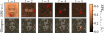
\includegraphics[scale=1]{figs/nogs/entropy-maps-2}
  \caption{A near-optimal glimpse sequence being generated for the task of
    inferring the attribute `Male'. \textbf{Top row:} A heatmap of the estimated
    expected posterior entropy for each possible next glimpse location $l_t$.
    The red cross marks the minimum, which is chosen as the next glimpse
    location. \textbf{Bottom row:} Red squares mark the observed parts of the
    image after each glimpse, and the rest is shown in grayscale. Even after 5
    glimpses, only 2.6\% of image pixels are observed. }
  \label{fig:epe-maps}
\end{figure*}

\section{Bayesian Optimal Experimental Design} \label{sec:nogs-boed} Designing an
experiment to be maximally informative is a fundamental problem that applies as
much to tuning the parameters of a political survey~\cite{warwick1975sample} as
to deciding where to direct attention to answer a query.
BOED~\cite{chaloner1995bayesian} provides a unifying framework for this problem
by allowing a formal comparison of possible experiments under problem-specific
prior knowledge.
%
Consider selecting the design, $l$, of an experiment to infer some unknown
parameter, $\theta$. For example, $\theta$ may be the median lethal dose of a
drug, and $l$ the doses of this drug given to various groups of
rats~\cite{chaloner1995bayesian}. Alternatively, as we consider in this paper,
$\theta$ is the class label of an image and $l$ determines which part of the
image we observe.
%
The experiment results in a measurement of $\y \sim p(\cdot|l, \theta)$. Following
the previous examples, $\y$ could be the number of rats which die in each group
or the observed pixel values. Given a prior distribution over $\theta$ and
knowledge of $p(\y|l, \theta)$, we can use the measurement to infer a posterior
distribution over $\theta$ using Bayes' rule: $p(\theta|\y,l) = \frac{p(\y|l,
  \theta)p(\theta)}{\int p(\y|l, \theta)p(\theta) \mathrm{d}\theta}$.
The aim of our experiment is to infer $\theta$, and so a well designed
experiment will reduce the uncertainty about $\theta$ by as much as possible.
The uncertainty after the experiment can be quantified by the Shannon entropy in
the posterior,
\begin{equation}
  \label{eq:pe}
  \entropy \left[ p(\theta | \y, l) \right] = \EX_{p(\theta | \y, l)} \left[ - \log p(\theta | \y, l) \right].
\end{equation}
To maximally reduce the uncertainty, we wish to select $l$ to minimise this
posterior entropy. However, the design of the experiment must be chosen before
$\y$ is measured and so we cannot evaluate the posterior entropy exactly.
Instead, we minimise an expectation of it over $p(\y|l)=\EX_{p(\theta)}\left[
  p(\y|l, \theta) \right]$, the marginal distribution of $\y$. This is the
expected posterior entropy, or $\EPE$,
\begin{align}
  \label{eq:epe}
  \text{EPE} (l) &= \EX_{p(\y|l)} \left[ \entropy \left[ p(\theta | \y, l) \right]  \right].
\end{align}
\Cref{eq:epe} is a criterion for selecting a one-off design for an experiment,
such as taking a single glimpse. For the case where a sequence of glimpses can
be taken, we need \textit{sequential} experimental design. In this scenario, the
choice of design $l_t$ can be informed by the designs and outcomes of previous
experiments, $l_{1:t-1}$ and $\y_{1:t-1}$. The marginal distribution over
outcomes is therefore $p(\y_t|l_{1:t},\y_{1:t-1})$ rather than $p(\y_t|l_t)$.
Similarly, the posterior after observing $\y_t$ is $p(\theta|l_{1:t},\y_{1:t})$.
%
We can therefore compute the EPE for the $t$th experiment as
%
% Therefore, in the sequential case which we consider throughout the rest of the
% paper, we greedily minimise the following form of the $\EPE$ on each iteration:
\begin{align}
  \label{eq:seq-epe}
  \text{EPE}_{\y_{1:t-1}, l_{1:t-1}} (l_t) = \EX_{p(\y_t | \y_{1:t-1}, l_{1:t})} \left[\entropy \left[ p(\theta | \y_{1:t}, l_{1:t} ) \right]  \right].
\end{align}
In this paper, as in many other BOED applications, we make sequential BOED
tractable by using a greedy minimisation~\cite{foster2019variational}. That is,
at each time $t$, we select
$l_t = \argmin{}_{l_t} \text{EPE}_{\y_{1:t-1}, l_{1:t-1}} (l_t)$, minimising the
EPE after the single next time step. We then perform the experiment with design
$l_t$ to observe $\y_t$ and repeat for $t=1,\ldots,T$.

\section{Generating Supervision Sequences} \label{sec:nogs-generating-seqs} To
reiterate the outline of our method, we first annotate a portion of the training
data with supervision sequences, describing a series of `good' locations to
attend to for each image. These supervision sequences can then speed up the
later training of hard attention networks. This section details how to generate
supervision sequences using either a trained hard attention network
(\cref{sec:nogs-rams}) or BOED (\cref{sec:nogs-nogs}).

\subsection{Sequences From a Trained Network} \label{sec:nogs-rams} One way to create
supervision sequences is to first train a network without supervision sequences.
We do so using the method suggested by \cite{mnih2014recurrent} for training the
`Recurrent Attention Model' (RAM). We then run this network on a subset of the
training data and record the sequence of locations $l_{1:T}$ it attends to on
each image $\x$.

\subsection{Near-optimal Glimpse Sequences}  \label{sec:nogs-nogs}

In \cref{sec:nogs-experiments} (and \cref{fig:glimpses} in particular), we find that
RAM networks can learn apparently sub-optimal sequences of glimpse locations. It
is also unclear how well supervision sequences produced using a particular RAM
architecture will generalise when used to train different hard attention
architectures. In this section, we therefore introduce our method to generate
supervision sequences using BOED. This method is agnostic to the choice of hard
attention architecture and, empirically, focuses attention on intuitive
locations (\cref{fig:glimpses}).

\ourparagraph{EPE estimator}
BOED requires a probabilistic model of the measurements and parameters we wish
to infer. That is, we need to define $p(\theta, \y_{1:t} | l_{1:t})$ for any
$l_{1:t}$. To do so in the visual attention setting, we first define $p(\theta,
\x)$ to be the intractable joint distribution over labels and images from which
our training and test data originate. %
%
To be consistent with our definition in \cref{sec:nogs-hard-attention} of $\y$ as a
deterministic function of $\x$ and $l$, we then define $p(\y_i|\x,l_i)$ to be a
Dirac-delta distribution on $\fovea(\x,l_i)$.
%
The joint distribution is then
\begin{equation} \label{eq:p-joint}
  p(\theta, \y_{1:t}|l_{1:t}) = \int p(\theta, \x) \prod_{i=1}^t p(\y_i|\x,l_i) \mathrm{d}\x.
\end{equation}
Given this joint distribution, $\text{EPE}_{\y_{1:t-1}, l_{1:t-1}} (l_t)$ is
well defined but intractable in general. We therefore consider how to
approximate it. To simplify our method for doing so, we first rearrange the
expression given in \lref{eq:seq-epe} so that the expectation is over $\x$
rather than $\y_t$. Taking advantage of the fact that $\y_i$ is a deterministic
function of $\x$ and $l_i$ allows it to be rewritten as follows (proof in the
appendix\footnote{We host an anonymised appendix at
  \url{https://drive.google.com/file/d/1MppBs8USo2iMI-yvUZV_DXUiPzF-4PhM}.}).
Defining $\fovea(\x, l_{1:t}) = \{ \fovea(\x, l_{1}),\ldots,\fovea(\x, l_t) \}$,
\begin{align} \label{eq:image-epe}
  \text{EPE}_{\y_{1:t-1}, l_{1:t-1}} (l_t) = \EX&_{p(\x | \y_{1:t-1}, l_{1:t-1})} \Big[ \nonumber\\
                                                &\entropy \left[ p(\theta | \fovea(\x, l_{1:t}), l_{1:t} ) \right]  \Big].
\end{align}
Given this form of the expected posterior entropy, we can approximate it if we
can leverage the dataset to obtain:
\begin{itemize}[itemsep=0pt, topsep=0pt]
\item a learned \textit{attentional variational posterior}, $\gavp(\theta | \y_{1:t}, l_{1:t} )
  \approx p(\theta | \y_{1:t}, l_{1:t} )$,
\item and \textit{stochastic image completion} distribution
  $\rimg(\x|\y_{1:t-1},l_{1:t-1}) \approx p(\x|\y_{1:t-1},l_{1:t-1})$.
\end{itemize}
We expand on the form of each of these approximations later in this section.
First, combining them with \cref{eq:image-epe} and using a Monte Carlo estimate
of the expectation yields our estimator for the $\EPE$. Given $\x^{(1)},\ldots,\x^{(N)} \sim \rimg(\cdot|\y_{1:t-1},l_{1:t-1})$,
\begin{align} \label{eq:approx-epe}
  \text{EPE}&_{\y_{1:t-1}, l_{1:t-1}} \left( l_{t} \right) \nonumber\\ &\approx \frac{1}{N} \sum_{n=1}^N \entropy \big[ \gavp(\theta | \fovea(\x^{(n)}, l_{1:t}), l_{1:t} ) \big] .
  %&\quad \text{with} \quad \x^{(1)},\ldots,\x^{(N)} \sim \rimg(\cdot|\y_{1:t-1},l_{1:t-1}) .
\end{align}
% with $\x^{(1)},\ldots,\x^{(N)} \sim \rimg(\x|\y_{1:t-1},l_{1:t-1})$.

\ourparagraph{Overview of BOED pipeline} We use a grid search to find the value
of $l_t$ which minimises \cref{eq:approx-epe}. That is, denoting the set of
allowed values of $l_t$ as $L$, we compute our approximation of
$\text{EPE}_{\y_{1:t-1}, l_{1:t-1}} (l_t)$ for all $l_t \in L$ and select the
value of $l_t$ for which this is least. To do so, our full BOED pipeline is:
\begin{enumerate}[itemsep=0pt, topsep=0pt]
\item Sample $\x^{(1)}\ldots,\x^{(N)} \sim \rimg(\cdot|\y_{1:t-1},l_{1:t-1})$.
\item For each $l_t \in L$, approximate the expected posterior entropy with
  \lref{eq:approx-epe}.
\item Select the value of $l_t$ which minimises \cref{eq:approx-epe}.
\end{enumerate}
Repeating these steps for $t = 1,\ldots,T$ yields a near-optimal glimpse
sequence $l_{1:T}$ for image $\x$. \Cref{fig:epe-maps} shows an example of this
process. In our experiments, we generate 600 to 1000 near-optimal glimpse sequences for each
dataset before using them to partially supervise hard attention training as
described in \cref{sec:nogs-sup}. We now describe the form of $\gavp$ (the
attentional variational posterior) and $\rimg$ (stochastic image completion).

\ourparagraph{Attentional variational posterior} In this section we introduce
our novel approach for efficiently approximating the intractable posterior
$p(\theta | \y_{1:t}, l_{1:t})$. We train a convolutional neural network (CNN)
to map from a sequence of glimpses $\y_{1:t}$ and their locations $l_{1:t}$ to
$\gavp(\theta | \y_{1:t}, l_{1:t})$, an approximation of this posterior. We call
this the attentional variational posterior CNN (AVP-CNN). To allow a single CNN
to cope with varying $\y_{1:t}$, $l_{1:t}$, and even varying $t$, we embed its
input as shown in \lref{fig:dropout-cnn}. We embed $l_{1:t}$ by creating an
image-sized mask which is 1 for observed pixels and 0 for unobserved pixels.
Elementwise multiplication of this mask with the input image sets unobserved
pixels to zero. The mask is then concatenated as an additional channel. This
embedding naturally maintains spatial information while enforcing an invariance
to permutations of the glimpse sequence. We use a
Densenet-121~\cite{huang2017densely} CNN architecture (pretrained on
ImageNet~\cite{imagenet}) to map from this embedding to a vector of
probabilities representing $\gavp$. We train the network to minimise the KL
divergence between its output and $p(\theta|\y_{1:t},l_{1:t})$. That is,
$D_{KL} \left( p(\theta|\y_{1:t},l_{1:t}) || \gavp(\theta|\y_{1:t},l_{1:t}) \right) $.
To ensure that $\gavp$ is close for all $t$, $l_{1:t}$ and $\y_{1:t}$, the loss
used is an expectation of this KL divergence over
$p(\y_{1:t}|l_{1:t})u(t, l_{1:t})$. We factorise $u(t, l_{1:t})$ as
$u(t)\prod_{i=1}^tu(l_i)$ where, so that all times and glimpse locations are
weighted equally in the loss, $u(t)$ is a uniform distribution over $1,\ldots,T$
and $u(l_i)$ is a uniform distribution over all image locations. Denoting the
network parameters $\lambda$, the gradient of this loss is
\begin{align} \label{eq:dropout-cnn-gradient}
  \frac{\partial}{\partial\lambda} \mathcal{L}_\lambda = \EX_{p(\theta, \y_{1:t}|l_{1:t})u(t, l_{1:t})} \left[ - \frac{\partial}{\partial\lambda} \log g_\text{AVP}^{\lambda}(\theta | \y_{1:t}, l_{1:t}) \right].
\end{align}
This gradient is the same as that of a cross-entropy loss on data sampled from
$p(\theta, \y_{1:t}|l_{1:t})u(t, l_{1:t})$, and can be approximated by a Monte
Carlo estimate.

\begin{figure}
  \centering
  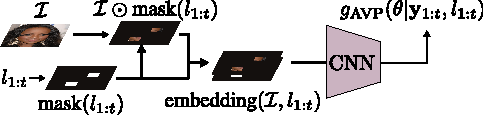
\includegraphics[scale=1]{figs/nogs/dropout-cnn}
  \caption{Attentional variational posterior CNN. An image and $l_{1:t}$ are
    processed to create an embedding of the information gained from glimpses $1$
    to $t$. An image classifier maps from this to an approximation of
    $p(\theta|\y_{1:t}, l_{1:t})$.}
  \label{fig:dropout-cnn}
\end{figure}

\begin{figure*}[t]
  \centering
  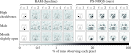
\includegraphics[scale=0.8]{figs/nogs/some-glimpses}
  \caption{Comparison of glimpse locations chosen by \RAM{} and \PSNOGS{} on the
    CelebA-HQ test set for three classification tasks. For each $t \in
    \{1,2,3,4,5\}$, we show an image where each pixel's colour corresponds to
    how often it was observed at this time step during testing. The outlines are
    produced by averaging outputs from a face detector across the dataset. For
    $t=1$, each network learns a single location which it attends to on every
    test image. This is expected behaviour as the first location is chosen
    before taking any glimpses, and therefore before being able to condition on
    the image. \RAM{} appears to then fail to learn to direct the later
    glimpses, attending almost uniformly across the image. In contrast,
    \PSNOGS{} distributes these glimpses broadly over the salient regions. }
  \label{fig:glimpses}
\end{figure*}

Our approximation of the $\EPE$ in \cref{eq:approx-epe} involves the entropy of
$\gavp$. Since $\gavp$ is a categorical distribution, this is simply computed
analytically. This amortised approximation of the posterior entropy is inspired
by \cite{foster2019variational}, but has two important differences to their
estimator:
\begin{itemize}[itemsep=0pt, topsep=0pt]
\item \cite{foster2019variational} learn a mapping from $\y_t$ to
  $g(\theta | \y_{1:t}, l_{1:t})$, sharing information between ``nearby''
  samples of $\y_t$ to reduce the computational cost of the experimental design.
  Our AVP-CNN takes this amortization further by learning a single mapping from
  $t$, $l_{1:t}$ and $\y_{1:t}$ to $\gavp(\theta | \y_{1:t}, l_{1:t})$, which
  yields significant further efficiency gains in our setting.
\item Whereas we approximate $\entropy[p]$ with $\entropy[\gavp] = \EX_\gavp[-\log\gavp]$,
  \cite{foster2019variational} use $\EX_p[-\log g]$. This provides an
  upper bound on $\entropy[p]$ but is not applicable in our case as we cannot
  sample from $p(\theta|\y_{1:t}, l_{1:t})$. Both approximations are exact when
  $\gavp = p$.
\end{itemize}

\ourparagraph{Stochastic image completion}
\label{sec:nogs-image-sampling}
We considered numerous ways to form $\rimg(\x | \y_{1:t-1}, l_{1:t-1})$
including inpainting~\cite{pathak2016context,isola2017image} and Markov chain
Monte Carlo in a generative model. Future research in generative modelling may
provide alternatives to this component of our method but, for now, we
represent $\rimg$ using a technique we developed based on image
retrieval~\cite{jegou2010improving}. Of the methods we considered, this gave the
best trade-off between speed, sample quality, and sample diversity. It involves creating an
empirical image distribution with 1.5 million images for each experiment using
GANs with publicly available pre-trained weights
(StyleGAN~\cite{karras2018style} for CelebA-HQ and
FineGAN~\cite{singh2019finegan} for Caltech-UCSD Birds). We note that the use of
pre-trained models makes test leakage possible but verify in the appendix that
this is unlikely to impact our results. During sampling, the database is
searched for images that `match' the previous glimpses ($\y_{1:t-1}$ and
$l_{1:t-1}$). How well these glimpses match a database image, $\x'$, is measured
by the squared distance in pixel space at glimpse locations:
$\sum_{i=1}^{t-1} \norm{\y_i - \fovea(\x', l_i)}^2_2$. This distance defines a
probability distribution over the images in the database.
%
To reduce computation, we first compare approximations of the observed parts of
each image using principal component analysis~\cite{jolliffe2011principal}, and
compute exact distances only when these are close. The overall procedure to
sample from $\rimg$ corresponds to importance
sampling~\cite{arulampalam2002tutorial} in a model where $p(\y_t | \x, l_t)$ is
relaxed from a Dirac-delta distribution to a Gaussian (details in appendix).

\begin{figure*}
  \centering
  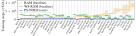
\includegraphics[scale=1]{figs/nogs/celebhq-training-time}
  \vspace{-.2cm}
  \caption{Number of training iterations before a validation cross-entropy loss
    within 0.01 of the best is achieved for each CelebA-HQ attribute (sorted by
    mean training time). On average, \PSNOGS{} trains almost $7\times$ faster
    than \RAM{}, the fastest baseline. \PSNOGS{} and \PSRAM{} both also exhibit
    greatly reduced variance in the training time.}
  \label{fig:celebhq-time}
  \vspace{-.3cm}
\end{figure*}

\section{Training with Partial Supervision} \label{sec:nogs-sup}
\label{sec:nogs-partially-supervised-training}
The previous section describes how to annotate an image with supervision
sequences for a particular image classification task. This section assumes that
such supervision sequences exist for all, or some, images in a dataset. These
can then be used to partially supervise the training of a hard attention
mechanism. We use separate losses for supervised (i.e. annotated with both a
class label and a sequence of glimpse locations) and unsupervised (i.e.
annotated with a class label but not glimpse locations) examples. By minimising
the sum of these losses, our procedure can be viewed as maximising the joint
log-likelihood of the class labels and supervision sequences. To be precise, let
$q_\phi (\theta^i, l_{1:T}^i | \x^i)$ be a network's joint distribution over the
chosen glimpse locations and predicted class label on image $\x^i$. Let $q_\phi
(\theta^i | \x^i)$ be the marginalisation of this distribution over $l^i_{1:t}$.
We maximise a lower bound on
\begin{equation}
  \label{eq:objective}
  \mathbf{L} = \sum_{i \in \text{sup.}} \overbrace{\log q_\phi (\theta^i, l_{1:T}^i | \x^i)}^{\text{supervised objective}} + \sum_{i \in \text{unsup.}} \overbrace{\log q_\phi (\theta^i | \x^i)}^{\text{unsupervised objective}}.
\end{equation}
where `sup' is the set of training indices with supervision sequences, and
`unsup' is the remainder. When running on unsupervised examples, we follow
\cite{mnih2014recurrent} and train the location network with a REINFORCE
estimate of the gradient of the accuracy, using a learned baseline to reduce the
variance of this estimate. Meanwhile, all other network components are trained
to maximise the log-likelihood of the class labels (i.e. minimise a
cross-entropy loss). \cite{ba2014multiple} noted that this maximises a lower
bound on the unsupervised objective in \lref{eq:objective}. For examples with
supervision sequences, the supervised objective in \lref{eq:objective} is
maximised by gradient backpropagation. The loss is computed by running the
network with its glimpse locations fixed to those in the supervision sequence.
The location network is updated to maximise the probability of outputting these
locations while, as for unsupervised examples, the other network modules are
trained to maximise the likelihood of the class labels. Minibatches can contain
both supervised and unsupervised examples, with gradients computed
simultaneously. We emphasise that supervision sequences are used throughout
training. Although it is common to attenuate such supervision signals so that an
end-to-end loss eventually dominates, preliminary experiments showed no
improvements from this.

\section{Experiments and Results} \label{sec:nogs-exp}
\label{sec:nogs-experiments}
\ourparagraph{Datasets and network architectures}
%
We test our approach on CelebA-HQ~\cite{karras2017progressive} and a cropped
variant of Caltech-UCSD Birds (CUB)~\cite{wah2011caltech}. For both, GANs exist
which satisfy the requirement to have a convincing generative
model~\cite{karras2018style,singh2019finegan}. The RNN is a
GRU~\cite{cho2014learning} and we use a simple classifier and location network
architecture (see the appendix for details). For both
datasets, we use $T=5$. The dataset-specific details are as follows: \textbf{(1)
  CelebA-HQ} Our experiments tackle 40 different binary classification tasks,
corresponding to the 40 labelled attributes. We resize the images to $224 \times
224$ and use training, validation, and test sets of $27\,000$, $500$, and $2500$
images respectively. We use $16\times16$ pixel glimpses, with a $50\times50$
grid of allowed glimpse locations. The glimpse network has two convolutional
layers followed by a linear layer. \textbf{(2) CUB} We perform 200-way
classification of bird species. We crop the images using the provided bounding
boxes and resize them to $128 \times 128$. Cropping is necessary because good
generative models do not exist for the uncropped dataset, but there is still
considerable variation in pose after cropping. We use 5120 training images, a
validation set of 874 and a test set of 5751 (having removed 43 images also
found in ImageNet). We use $32\times32$ pixel glimpses and a $12\times12$ grid
of allowed glimpse locations so that adjacent locations are 8 pixels apart. The
glimpse network is the first 12 convolutional layers of a VGG pretrained on
ImageNet~\cite{simonyan2014very, imagenet}.

\begin{figure}
  \centering
  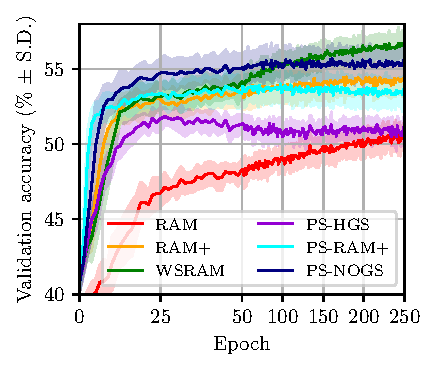
\includegraphics[scale=1]{figs/nogs/birds-training-avg}
  \vspace{-.4cm}
  \caption{CUB validation accuracy over training. }
  \vspace{-.4cm}
  \label{fig:birds-training}
\end{figure}

\ourparagraph{Generating supervision sequences} We create $600$ near-optimal
glimpse sequences for each of the 40 CelebA-HQ classification tasks, and $1000$
for CUB. This is a one-off computation that need only be done once for a
particular task. It took 20 GPU-hours for CUB, and 10 GPU-days for each
CelebA-HQ task. We publicly release these sequences along with our
code\footnote{\url{https://drive.google.com/file/d/1LS-0U7wRQOqyKn2QECocNlyPhSY8wRAT}},
allowing them to be re-used by anyone to speed up the training of hard attention
networks on these tasks. We test \PSRAM{} on each task using the same number of
supervision sequences as \PSNOGS{} (i.e. 1000 for CUB and 600 for each CelebA-HQ
task).

\ourparagraph{Baselines} All methods we compare use the same neural
architecture; only the training algorithm is varied. For each experiment we
compare against the \RAM{} algorithm \cite{mnih2014recurrent}, which is
equivalent to the special case of our partially supervised objective with zero
supervision sequences.
%
We also compare against training with wake-sleep
(\WSRAM{})~\cite{ba2015learning}, which we describe in \cref{sec:nogs-related-work}.
Furthermore, we compare against supervising training with ``hand-crafted glimpse
sequences'' (\HGS{}) on CUB. These are designed, using CUB's hand-annotated
features, to attend to the beak, eye, forehead, belly and feet (in that order).
If any of these parts are obscured, they are replaced by a randomly selected
visible body part. We annotate the same number of images for this baseline as
for \PSRAM{} and \PSNOGS{}. We have not observed significant performance
improvements from varying this number.

\ourparagraph{Partial-supervision for CelebA-HQ} In \lref{fig:celebhq-time}, we
plot the number of iterations until convergence on each CelebA-HQ classification
task. On almost all tasks, the methods which involve partial supervision
(\PSRAM{} and \PSNOGS{}) are faster than those which do not. \Cref{tab:results}
corroborates this finding, showing that \PSNOGS{} trains an average of
$6.6\times$ faster on CelebA-HQ than \RAM{}, the fastest unsupervised method.
Furthermore, the test accuracy for the partially supervised methods is
competitive with the unsupervised baselines. \lref{fig:glimpses} compares the
learned attention policies for several tasks, with the remainder in the
appendix. Unlike \RAM{}, \PSNOGS{} appears to learn a suitable policy at every
time step. These intuitively reasonable policies may explain why \PSNOGS{}
trains $20\%$ faster than \PSRAM{} on CelebA-HQ.

\begin{table}
  \caption{Iterations to convergence and test accuracy for each method and
    dataset. Our methods are marked with {$^*$}. The first row corresponds to
    \RAM{} on CelebA-HQ and \RAMP{} on CUB.}
  \vspace{-.1cm}
  \label{tab:results}
  \centering
  \begin{tabular}{lllll}
    \toprule
    \multicolumn{1}{r}{} & \multicolumn{2}{c}{CelebA-HQ (avg.)} & \multicolumn{2}{c}{CUB}                 \\
    \cmidrule(r){2-3} \cmidrule(r){4-5}
    Method     & Iterations & Acc. (\%)  & Iterations & Acc. (\%)  \\
    \midrule
    \RAM{}(+)     & 25\,100     & 87.1           & 5690           & 53.7          \\
    \WSRAM{}             & 40\,700     & {88.1}         & 11\,800        & {55.7}        \\
    \HGS{}               & -           & -              & {1790}         & 50.5          \\
    \PSRAM{}(+)$^*$      & 4750        & 87.0           & 1980           & 53.2          \\
    \PSNOGS{}$^*$        & {3820}      & 87.0           & 3530           & 54.4          \\
    \bottomrule
  \end{tabular}
  \vspace{-.2cm}
\end{table}


\ourparagraph{Partial-supervision for CUB} On CUB, a pretraining stage is
necessary to achieve high accuracy. We therefore pretrain the classifier, RNN,
and glimpse network with glimpse locations sampled independently at each time
step from either a uniform distribution (in the case of \RAM) or from a
heuristic which assigns higher probability to more salient locations, as
estimated using the AVP-CNN (\RAMP{} and all others). See the
appendix for details.
% convergence measured by first valid. acc. within 1% of best valid. acc.
% ceil(5120/64)=80 iterations per epoch
\Cref{fig:birds-training} shows the validation accuracy of each method
throughout training.
%
As seen on CelebA-HQ, all methods with partial supervision train faster than any
without; \cref{tab:results} show the number of iterations on CUB before
achieving a validation accuracy within 1\% of the highest. Of the methods with
partial supervision, \HGS{} quickly saturates and achieves the lowest test
accuracy of the methods we compare. \PSRAMP{} achieves slightly lower accuracy
than \RAMP{}, whose policy it is trained to imitate. \PSNOGS{} achieves the
highest accuracy of the partially supervised methods, indicating that
near-optimal glimpse sequences are more suitable for training than any of the
supervision sequences used by our baselines. The methods with partial
supervision outperform methods without for the first 100 training epochs,
providing further evidence that partial supervision speeds up training. After
this point, \WSRAM{} achieves higher validation accuracy than \PSNOGS{}. This
may be due to some bias introduced by approximations in the generation of
near-optimal glimpse sequences, which will not go away with further training.

\section{Neural Architecture Search} \label{sec:nogs-nas}
% Our NAS objective trades off accuracy and computation, resulting in a set of
% architectures suited to low-power computation. We show that hard attention
% networks with these architectures can outperform networks which process the
% whole image when matched to use the same low number of floating point operations
% (FLOPs). We perform NAS independently to find architectures for 5 CelebA-HQ
% binary classification tasks.

In this section we describe a neural architecture search (NAS) over hard
attention network architectures. The optimised architectures could, for some
tasks and when matched to use the same number of floating point operations
(FLOPs), outperform CNNs with access to the whole image.
% In this section, we show the results of a neural architecture search (NAS) for
% hard attention network architectures.
%
To speed up the training of each architecture during NAS, and therefore allow
more architectures to be evaluated, we train them with \PSNOGS{}. We select
architectures to evaluate using Bayesian optimisation, and use the Hyperband
algorithm~\cite{li2017hyperband} to quickly halt non-promising runs based on
their performance early in training. We perform independent architecture
searches for 5 different CelebA-HQ classification tasks; each use 25 days of
computation. To describe an example NAS (for the task of inferring `Mustache'),
1385 hyperparameter settings in total were tested and trained for a maximum of
200 epochs. Due to Hyperband, all but 65 were stopped before reaching 25 epochs.
Our NAS objective is $acc - 2 \cdot \log n_\text{FLOPs}$, where $acc$ is the
best percentage validation accuracy achieved throughout training and
$n_\text{FLOPs}$ is the number of FLOPs performed over the course of $T=5$
glimpses. Since we observed that \WSRAM{} achieves higher accuracy after
sufficient training time, we take up to seven of the best architectures (in
terms of validation accuracy) and retrain them with \WSRAM{}. As an additional
innovation to minimise the power usage, we modify the network architecture to
allow it to stop after fewer than $T$ glimpses when it is sufficiently certain.
This involves training a different classifier to use at each time step, and a
network which maps from the hidden state to the expected information gain from
the next glimpse. The network stops and makes a prediction whenever the expected
information gain for the next glimpse is below some threshold. See the appendix
for more details. The cyan lines in \cref{fig:acc-flops} show the test balanced
accuracies achieved by the chosen architectures with the stopping threshold
varied.
%
% We plot the balanced accuracy (the average accuracy over all classes)
% since the standard accuracy can be misleading for imbalanced classification.
%
We use CNN baselines based on ShuffleNetV2~\cite{ma2018shufflenet}, an
architecture designed for low-power performance. To adapt it to the extremely
low-power settings we deal with, we perform a grid search over three
hyperparameters: the input resolution; a multiplier for the number of
convolutional channels in each network layer; and the learning rate. We also
experimented with MobileNetV2~\cite{sandler2018mobilenetv2}, but found its
performance to be significantly worse than ShuffleNetV2 when adapted with these
hyperparameters. This resulted in a range of networks with varying accuracy and
computational requirements. We demonstrate the test accuracy-FLOPs trade-off
with the dashed line interpolating between the best-performing CNNs in
\cref{fig:acc-flops}. The CNNs shown in this line are selected based on their
validation accuracy. For the 2 tasks in \cref{fig:acc-flops}, hard attention is
clearly advantageous, achieving similar accuracy to the baselines with an order
of magnitude less computation. We note that this does not hold for all tasks,
and show 3 tasks in the appendix in which CNNs outperform hard attention
networks when more than about 0.5 MFLOPs are available. The advantage of
attention is clearly task-specific and may be improved with, e.g., different
glimpse sizes.

\begin{figure}[t]
  \centering
  \vspace{-.1cm}
  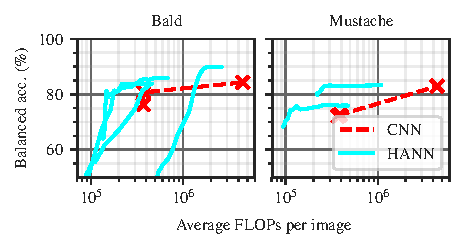
\includegraphics[scale=1]{figs/nogs/acc-flops-comparison-some}
  \vspace{-.2cm}
  \caption{Comparison of optimised low-power CNN architectures (red) with hard
    attention network, or HANN, architectures (cyan) found using \PSNOGS{}. The
    dashed red line interpolates between the best-performing CNN architectures.
    Each dashed blue line corresponds to a different HANN architecture. The HANN
    architectures can be tuned to any point along this line at test-time by
    setting a `stopping threshold' which trades off computation and accuracy.
    For these two attributes, and in the low-FLOP regime displayed, HANNs
    clearly outperform CNNs which process the entire image.}
    \vspace{-.3cm}
  \label{fig:acc-flops}
\end{figure}

\section{Related Work} \label{sec:nogs-related-work}

\ourparagraph{Variational approaches} A notable body of
work~\cite{ba2015learning,lawson2018learning,shankar2018posterior} frames the
glimpse locations as latent variables and trains an inference network to
approximate $q_\phi (l_{1:T} | \theta, \x)$. This improves estimates of the
objective $\log q_\phi (\theta | \x)$, which is marginalised over glimpse
locations. Our comparison against \WSRAM{}~\cite{ba2015learning} indicates that
using supervision sequences allows faster training than these variational
techniques alone. Further, supervision sequences could be used in conjunction
with these techniques~\cite{teng2020semi}.
% We emphasize that the framing of the problem
% using BOED is fundamentally different from that using variational inference:
% BOED aims to find the single optimal glimpse location at each step, whereas
% variational approaches sample from a distribution over `good' glimpse locations.

% another motivation for not processing full image: real sensors on robots
\ourparagraph{Models of hard attention} \cite{elsayed2019saccader} recently
demonstrated a hard attention network which achieved accuracy on
ImageNet~\cite{imagenet} close to that of CNNs which use the whole image.
However, their approach neccesitates running a convolutional network on the
entire image to select glimpse locations. As such, they advertise improvements
in interpretability rather than computational efficiency.
\cite{sermanet2014attention} train a hard attention architecture with REINFORCE
to achieve state-of-the-art accuracy on the Stanford Dogs dataset. In addition
to accessing the full image in low resolution at the start, they use large
glimpses (multiple $96\times96$ pixel patches at different resolutions) to
effectively solve the task in a single step. This avoids problems resulting from
learning long sequences with REINFORCE but also rules out the computational
gains possible with smaller glimpses. \cite{katharopoulos2019processing}
proposed a form of hard attention where, after processing the downsampled image,
multiple glimpses are sampled and processed simultaneously. This is again
incompatible with a low-power setting where we cannot afford to operate on the
full image.

% Elsayedo
% - needs full image

% Sermanet
% - needs full image
% - massive glimpses

% Katharop
% - needs full image
% - simultaneous

\ourparagraph{Supervised attention} We are not alone in providing supervision
targets for an attention mechanism. This is common for soft attention in visual
question answering, where targets have been created by human subjects, either
with gaze-tracking~\cite{yu2017supervising} or explicit
annotation~\cite{das2017human}. Either way is expensive and
dataset-specific~\cite{das2017human, gan2017vqs}. Recent work has reduced this
cost by e.g. extrapolating supervision signals from annotated datasets to other,
related, datasets~\cite{qiao2018exploring}, or using existing segmentations to
speed up annotation~\cite{gan2017vqs}. Even so, considerable human effort is
required. \PSNOGS{} automates this for image classification.


\section{Discussion and Conclusion}

We have demonstrated two methods for generating supervision sequences, and
introduced a partially supervised training objective which uses them to speed up
hard attention network training. \PSRAM{} is a simple way to speed up training,
while \PSNOGS{} gives bigger improvements for a greater up-front cost. We
release the near-optimal glimpse sequences generated to the public so that
faster training and experimentation on these tasks is possible without
generating new sequences. We also used the supervision sequences in a neural
architecture search, and demonstrated that the resulting low-power hard
attention networks can outperform CNNs which operate on the whole image. Future
work may extend our BOED framework to attention tasks such as question answering
where the latent variables are richly structured, or scale it using improved
generative models.
